\documentclass[UTF8]{ctexbeamer}
\usetheme{Madrid}
% \usecolortheme{beaver}
\usepackage{hyperref}
\usepackage{graphicx}
\usepackage{wrapfig}
\DeclareGraphicsExtensions{.eps,.ps,.jpg,.bmp,.png}

% \date{\today}
\title{Web基础}
% \subtitle{tutorial}

\author{紫丁香 CTF 俱乐部}

\date[Nov 2020]{November 2020}


\AtBeginSection[]
{
	\begin{frame}
		\frametitle{Table of Contents}
		\tableofcontents[currentsection]
	\end{frame}
}



\begin{document}
\frame{\titlepage}
\begin{frame}{在此之前}
    本 Slide 初始由紫丁香 CTF 俱乐部阮行止制作,于 2021-04-10 由Billchenchina以LaTeX重制。
    
    本 Slide 所有内容以\href{https://creativecommons.org/share-your-work/public-domain/cc0/}{CC0}授权进入公有领域。
\end{frame}
\begin{frame}{intro}
我是紫丁香CTF俱乐部的主席

您可以叫我,阮行止

曾经是OIer \& ACMer,从19年开始打CTF

主攻crypto和web

\end{frame}

\begin{frame}{本系列讲座是……}
    \begin{itemize}
        \item 开放的
        \item 面向零基础初学者的
        \item 实践的
        \item 尽量易于理解的
        \item 需要自学的
    \end{itemize}
\end{frame}
\begin{frame}{本系列讲座不是……}
    \begin{itemize}
        \item 覆盖所有知识的
        \item 完全严谨的
    \end{itemize}
\end{frame}


\begin{frame}
	\frametitle{Table of Contents}
	\tableofcontents
\end{frame}
\section{当我访问网站时,我在干些什么 - web概述}
\begin{frame}{浏览器}
    浏览器是我们访问网站的工具
    \begin{itemize}
        \item Google chrome
        \item Mozilla firefox
    \end{itemize}
    浏览器负责发送请求、渲染页面、etc.
\end{frame}
\begin{frame}{浏览器与服务器的交互}
    \begin{figure}
        \centering
        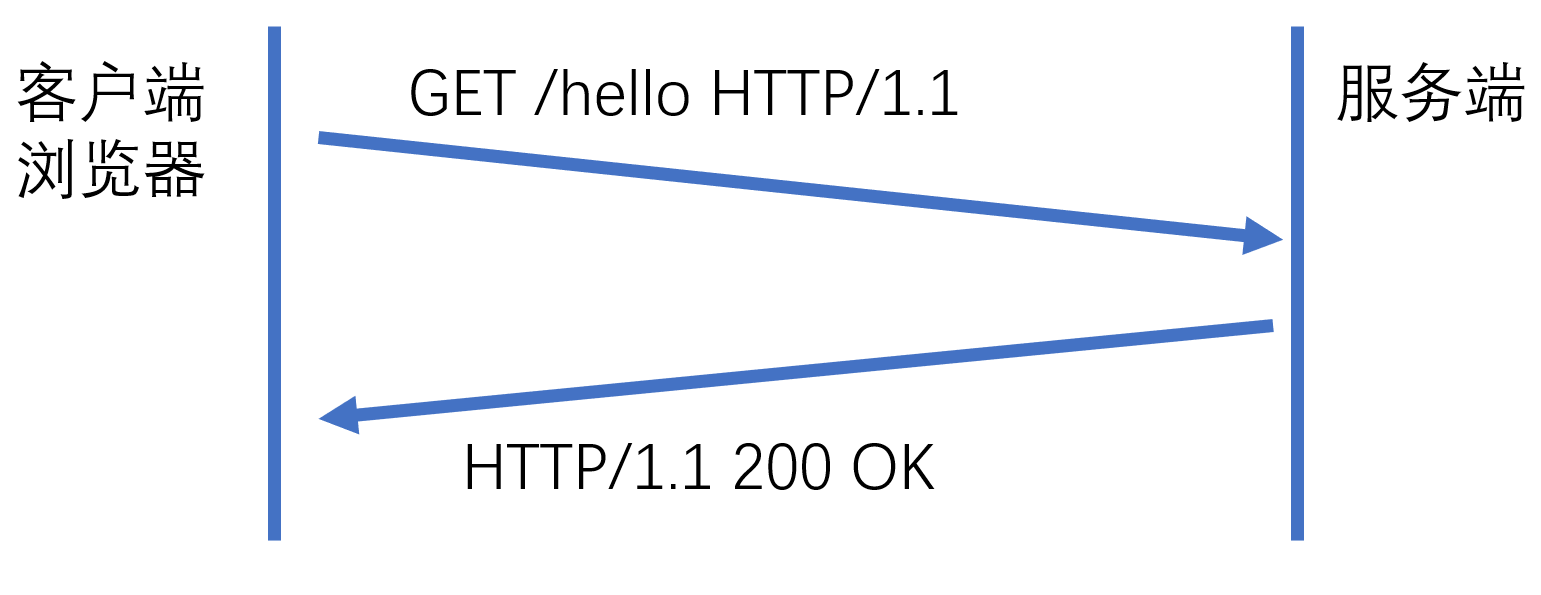
\includegraphics[width=0.8\textwidth]{http.png}
    \end{figure}
\end{frame}
\begin{frame}{C/S结构}
    web服务器是典型的 client/server 结构。
    
    有一台总是在线的服务器
    
    客户端向服务器发起请求(request)
    
    服务器接受请求,并发回响应(response)
\end{frame}
\begin{frame}{服务器}
    web中谈起服务器,往往指的是服务端程序
    \begin{itemize}
        \item nginx
        \item apache
        \item 其他,例如 python3 -m http.server
    \end{itemize}
\end{frame}
\begin{frame}{演示:搭建服务器}
    我将为各位演示搭建一个服务器的过程

    客户端访问 index.html 时,返回一句 hello

\end{frame}
\begin{frame}{URL}
    HTTP请求的“地址”,称为 URL
    \begin{itemize}
        \item http://www.baidu.com/index.html
        \item http://127.0.0.1/nana.php?id=3
        \item http://lilac.run:12345/
    \end{itemize}
\end{frame}
\begin{frame}{主机和端口}
    主机可以用域名或者 IP 地址来指定。
    
    端口号:0~65535 之间的一个数
    
    \vspace{2em}
    
    主机类似于一栋楼,端口号类似于房间号
    
    楼栋+房间号才能唯一定位到一个商户

\end{frame}
\begin{frame}{备注:域名}
    我们注意到,记忆IP地址是困难的。
    
    经常采用域名来代替冗长的IP地址。
    
    \vspace{1em}
    
    域名可以指向一个IP地址。
    
    详情请自学:DNS

\end{frame}
\begin{frame}{备注:端口}
    1000以下的端口号为周知端口号,我们约定
    \begin{itemize}
        \item 80端口用于HTTP服务
        \item 443端口用于HTTPS服务
        \item 22端口用于ssh服务
        \item etc.
    \end{itemize}

\end{frame}
\begin{frame}{浏览器如何渲染页面?}
    请打开 https://ruanx.net ,然后按F12
    
    \vspace{1em}
    
    请查阅:
    \begin{itemize}
        \item html
        \item javascript
        \item css
    \end{itemize}

\end{frame}
\begin{frame}{静态网站}
    静态网站类似于文件服务器
    
    请求一个路径,返回对应的文件
    
    无论谁访问,都会返回一样的文件
\end{frame}
\begin{frame}{静态网站}
    静态网站能不能实现一个简单的博客?
    
    \url{https://merrg1n.github.io/}
    
    静态网站能不能实现电子邮箱?
    
    静态网站能不能实现淘宝?

\end{frame}

\begin{frame}{动态网站}
    静态网站无法为用户提供个性化的服务。

    \vspace{2em}

    动态网站:由服务器上的程序计算出页面

\end{frame}

\begin{frame}{演示:动态网站}
    我将演示一个PHP服务器。
    
    访问 hello.php?username=nana
    
    将会返回 hello, nana!
    
\end{frame}

\begin{frame}{服务器后端程序}
    \begin{itemize}
        \item PHP
        \item Python(flask, django)
        \item nodejs(express)
        \item C/C++ CGI
        \item etc.
    \end{itemize}
\end{frame}
\begin{frame}{动态页面实现}
    以apache+php为例
    
    \begin{figure}
        \centering
        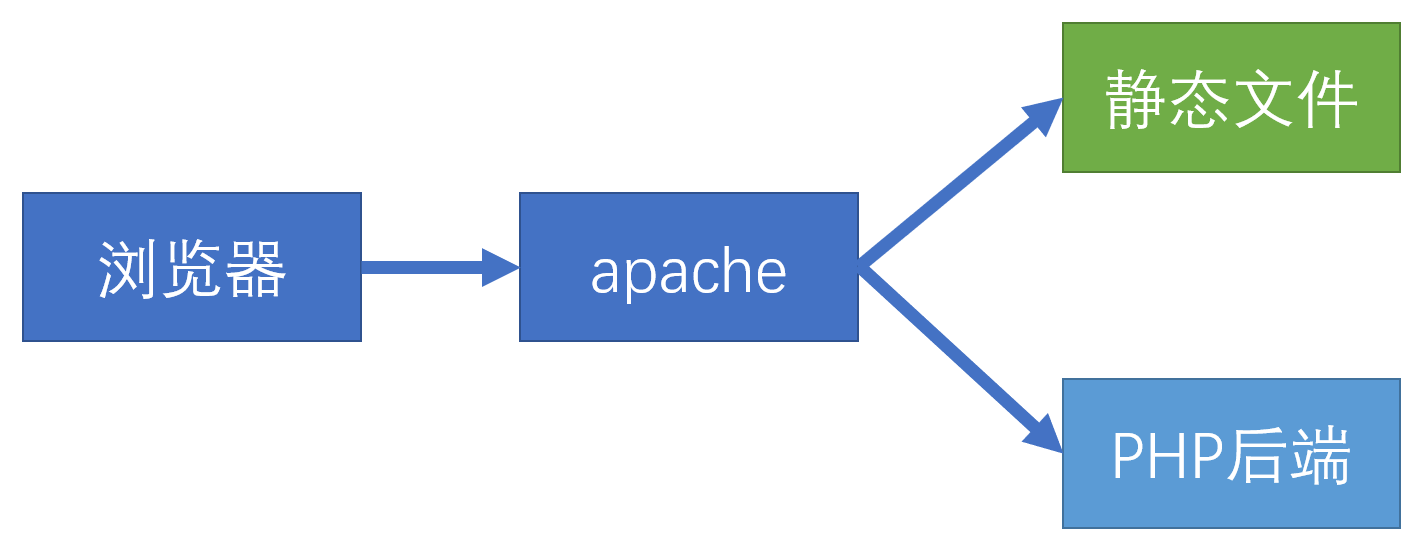
\includegraphics[width=0.8\textwidth]{dynamic.png}
    \end{figure}
\end{frame}

\section{浏览器如何与服务器交互 - 初步讨论HTTP协议}

\begin{frame}{实践:抓包}
    
    让我们看一看:
    
    \begin{itemize}
        \item 浏览器往服务器发送了什么内容
        \item 服务器返回了什么内容
    \end{itemize}
    
    工具:burp suite + SwitchyOmega
    
    另,开发者工具(F12)也可以完成简易的抓包

\end{frame}

\begin{frame}{HTTP协议}
    参阅:
    \begin{itemize}
        \item 《图解HTTP》(推荐)
        \item 《计算机网络:自顶向下方法》的HTTP部分
    \end{itemize}
\end{frame}
\begin{frame}[fragile]{HTTP请求实例}
    \begin{verbatim}
GET /somedir/page.html HTTP/1.1
Host: www.someschool.edu
Connection: close
User-agent: Mozilla/5.0
Accept-language: fr
\end{verbatim}
\end{frame}
\begin{frame}{请求格式}
    \begin{figure}
        \centering
        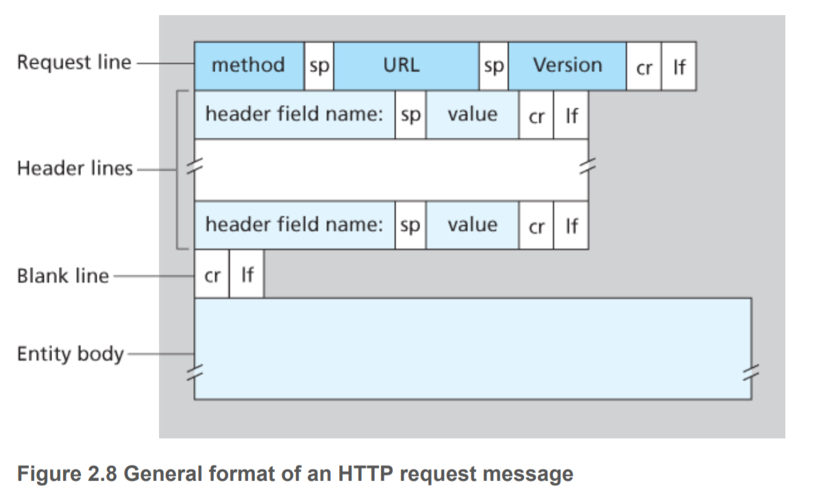
\includegraphics[width=0.9\textwidth]{http-request.png}
    \end{figure}
\end{frame}

\begin{frame}[fragile]{HTTP响应实例}
    \begin{verbatim}
HTTP/1.1 200 OK
Connection: close
Date: Tue, 18 Aug 2015 15:44:04 GMT
Server: Apache/2.2.3 (CentOS)
Last-Modified: Tue, 18 Aug 2015 15:11:03 GMT
Content-Length: 6821
Content-Type: text/html

Hello, world!
\end{verbatim}
\end{frame}

\begin{frame}{响应格式}
    \begin{figure}
        \centering
        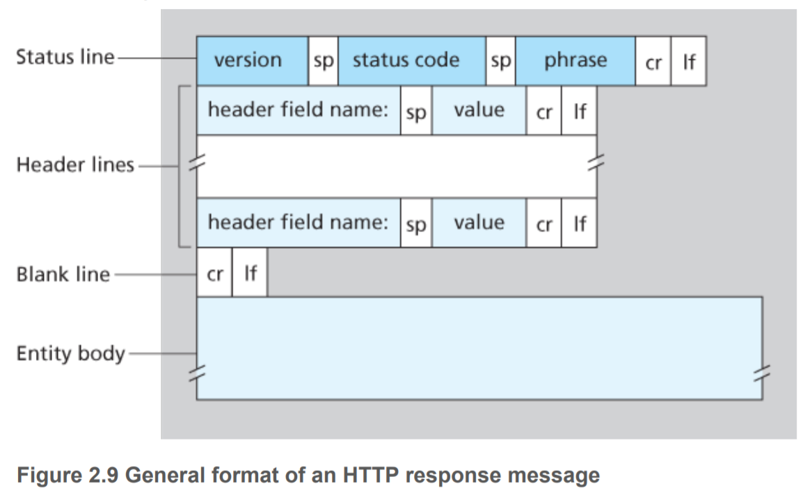
\includegraphics[width=0.9\textwidth]{http-response.png}
    \end{figure}
\end{frame}

\begin{frame}{注释:HTTP请求方法}
GET:一般用于不带参数或明文带参数的请求

POST:在GET的基础上,可以传输更大的参数,且POST上去的参数不显示在 URL

\vspace{1em}

在论坛中请求特定tag的帖子,用哪种请求?

传输文件,用哪种请求?

登录时传输用户名和密码,用哪种请求?

\end{frame}

\begin{frame}{演示:参数爆破}
    攻防世界 ics-06

    提示:报表中心,1~5000以内的某个id是特殊的

\end{frame}

\begin{frame}{注释:HTTP版本}
    总而言之,越高的版本越先进

    有兴趣的同学可参阅MDN文档

    \url{https://developer.mozilla.org/zh-CN/docs/Web/HTTP/Basics_of_HTTP/Evolution_of_HTTP}

\end{frame}

\begin{frame}{注释:响应状态码}
    状态码(status code)指示请求的结果
    
    \begin{itemize}
        \item 200 请求成功,一切正常
        \item 404 页面找不到
        \item 403 没有权限访问
        \item 503 服务器炸了
        \item 502/504 网关无效、网关超时(常见于proxy服务器)
    \end{itemize}
\end{frame}

\section{特殊的请求头 - 若干header讨论}
\begin{frame}{请求头}
    请求头(headers)用于提供一些的信息。
    
    CTF简单web题经常考察请求头相关的知识。
    
    \vspace{1em}
    
    可以通过Hackbar插件修改请求头。

\end{frame}

\begin{frame}{记录源IP的header}
    请求头中,可以有一些header指示源IP
    \begin{itemize}
        \item X-Forwarded-For
        \item X-Real-IP
    \end{itemize}
\end{frame}

\begin{frame}{实践:伪造源IP}
    Lilac Web Train平台: web.lilac.run

    用多种方式实现利用:

    \begin{itemize}
        \item Hackbar插件
        \item burp
        \item python requests
    \end{itemize}
\end{frame}

\begin{frame}{HTTP无状态性}

    HTTP是一个无状态协议。

    服务端程序不维护客户状态。

    每次请求,服务端仅能得到HTTP请求数据。
    
    \vspace{1em}
    
    如何实现一个购物车?
    
\end{frame}

\begin{frame}{Cookie}
    Cookie可以理解为由浏览器维护的一个记事本。
    
    对相同的网站进行访问时:
    
    \begin{itemize}
        \item 客户端浏览器每次请求都把自己维护的 Cookie 写进请求头
        \item 服务器可以通过 Set-Cookie 响应头,要求客户浏览器设置 Cookie
    \end{itemize}
\end{frame}

\begin{frame}{注释:Cookie的更多信息}
    详细信息请参阅MDN文档

    \url{https://developer.mozilla.org/zh-CN/docs/Web/HTTP/Cookies}

    Cookie带来了隐私性问题
\end{frame}
\begin{frame}{注释:Cookie的安全性}
    若网站开发者希望使用Cookie,但不想让用户知道Cookie里面的具体细节,有多种方式:
    \begin{itemize}
        \item 乞灵于密码学(先加密,再发给浏览器存储)
        \item Cookie中只存放这个用户的id,而由服务器后端来维护每个id对应的信息(PHP SESSION采取的方式)
    \end{itemize}
\end{frame}

\begin{frame}{实践:篡改Cookie}
    我们将通过篡改Cookie,把自己伪装成管理员。
    
    Lilac Web Train平台
    
    多种实现:
    \begin{itemize}
        \item Chrome浏览器原生cookie管理
        \item burp, Hackbar, python requests
    \end{itemize}    
\end{frame}
\begin{frame}{应对:防止用户篡改Cookie}
    借助SESSION ID,由后端维护用户状态 (PHP)
    
    Cookie存放密文数据
    
    Cookie存放明文数据+签名 (Flask)
\end{frame}
\begin{frame}{演示:PYWebsite}
    BUUOJ PYWebsite
    \begin{itemize}
        \item 前端验证
        \item 请求头伪造
    \end{itemize}
\end{frame}
\section{CTF web方向概述 - Let's dive in!}
\begin{frame}{web后端}
    
    国内赛事,多数题目是PHP后端
    
    有向python、nodejs、java转移的趋势
    
    越来越少考察PHP的奇技淫巧
    
    转而考察web与其他方向的综合

\end{frame}
\begin{frame}{web常见漏洞}
    
    SQL注入:拼接数据库操作字符串产生漏洞
    
    RCE:因某些不当原因,攻击者可以任意执行代码
    
    反序列化:将字符串解析成对象时的漏洞
    
    文件上传:一般是上传PHP webshell

\end{frame}
\begin{frame}{web常见漏洞}
    
    SSTI:服务端用模板引擎渲染攻击者提供的字符串
    
    XXE:XML解析漏洞
    
    XSS:向页面中注入恶意js代码,受害者浏览器访问页面
    
    etc.

\end{frame}

\begin{frame}{学习路线建议}
    \begin{itemize}
        \item Python(所有方向必须)
        \item PHP(web必须)
        \item HTML, js, css(了解即可)
        \item SQL(web必须)
        \item nodejs,java(可选)
    \end{itemize}
\end{frame}
\begin{frame}{本周学习推荐}
    在自己的 PC 上搭建 PHP 环境
    
    初步学习 PHP 语法(可考虑菜鸟教程)
    
    学习 python3 (建议搭建 anaconda 环境)廖雪峰 Python3 

\end{frame}

\section{结语}
\begin{frame}{结语}
    吾生也有涯,而知也无涯
    
    自学能力是CTF所有方向最重要的技能
    
    以有涯随无涯殆已,学习要有取舍
    
    共同努力,共同进步,请多与俱乐部会员交流
\end{frame}

\end{document}
